\documentclass{standalone}
\usepackage{tikz}
\usepackage{ctex,siunitx}
\setCJKmainfont{Noto Serif CJK SC}
\usepackage{tkz-euclide}
\usepackage{amsmath}
\usetikzlibrary{patterns, calc}
\usetikzlibrary {decorations.pathmorphing, decorations.pathreplacing, decorations.shapes,}

\begin{document}
\small
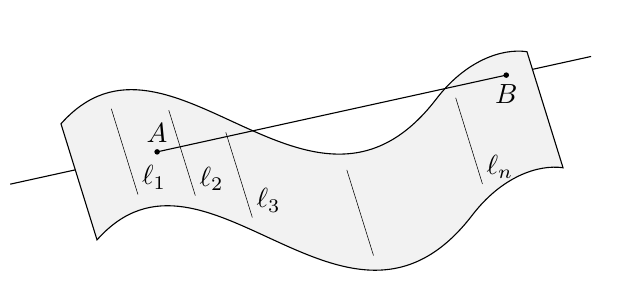
\begin{tikzpicture}[>=stealth,scale=1.0]
  \tkzSetUpPoint[fill=black]
  \useasboundingbox(-4,-1)rectangle(3.15,2.2);
  \draw[thin](-2.3561,0.6227)--(-4.2215,0.2125);
  \draw[thin](3.1550,1.8343)--(2.0780,1.5975);
  \draw[fill=gray!10](-3.577, 0.979)..controls(-2.194, 2.539)and(-0.394,-0.769)..( 1.190, 1.295)..controls( 1.561, 1.779)and( 2.020, 1.941)..( 2.341, 1.895)--( 2.799, 0.421)..controls( 2.479, 0.467)and( 2.019, 0.304)..( 1.648,-0.179)..controls( 0.064,-2.244)and(-1.735, 1.065)..(-3.119,-0.495)--cycle;
  \draw[very thin](-2.938, 1.170)--(-2.599, 0.080)node[pos=0.8,right]{$\ell_1$}
  (-2.208, 1.152)--(-1.871, 0.068)node[pos=0.8,right]{$\ell_2$}
  (-1.484, 0.872)--(-1.147,-0.210)node[pos=0.8,right]{$\ell_3$}
  ( 0.053, 0.394)--( 0.392,-0.693)
  ( 1.436, 1.309)--( 1.776, 0.215)node[pos=0.8,right]{$\ell_n$};
  \draw[thin](-2.3561,0.6227)--(2.0780,1.5975);
  \fill(-2.3561,0.6227)circle(1pt)node[above]{$A$};
  \fill(2.0780,1.5975)circle(1pt)node[below]{$B$};
\end{tikzpicture}
\end{document}